\section{Theorie}
\label{sec:Theorie}
\subsection{Hookesches-Gesetz}
Kräfte die an der Oberfläche eine Körpers angreifen und Gestalts- und Volumenveränderungen
hervorrufen, werden meist auf die Flächen bezogen und als Spannung bezeichnet.
Die senkrecht zur Oberfläche stehende Teil wird als Normalspannung $\sigma$ oder
Druck bezeichnet. Die Komponente die parallel zu der Oberfläche steht wird Tangential-
bzw. Schubspannung genannt. Das Hookesche Gesetz
\begin{equation}
  \sigma=E\frac{\Delta L}{L}
\end{equation}
beschreibt den, bei kleinen relativen Änderungen $\frac{\Delta L}{L}$, linearen
Zusammenhang zwischen Spannung und Deformation wie in Abbildung \ref{fig:Spannung}.
\begin{figure}[H]
  \centering
  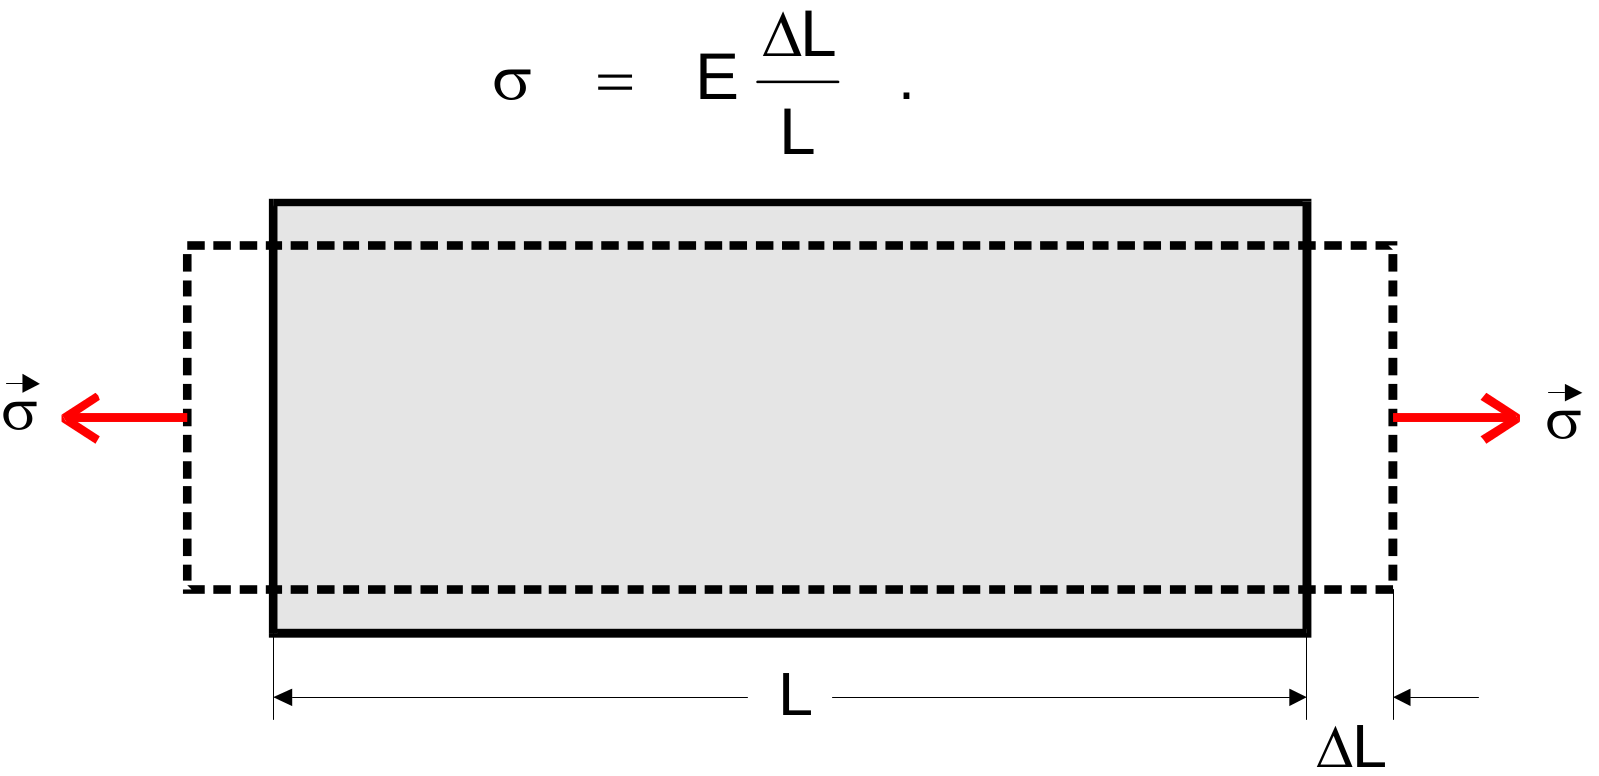
\includegraphics[width=0.7\textwidth]{spannung.png}
  \caption{Auswirkung einer Normalspannung auf eine stabförmige Probe \cite{sample} .}
  \label{fig:Spannung}
\end{figure}
Hierbei ist $E$ der Elastizitätsmodul, der eine Materialkonstante ist.

\subsection{Biegung bei einseitiger Einspannung}
In der Abbildung \ref{fig:Einseitige_Einspannung} ist, die schematische Darstellung
einer Biegung bei einseitiger Einspannung zu sehen.
\begin{figure}[H]
  \centering
  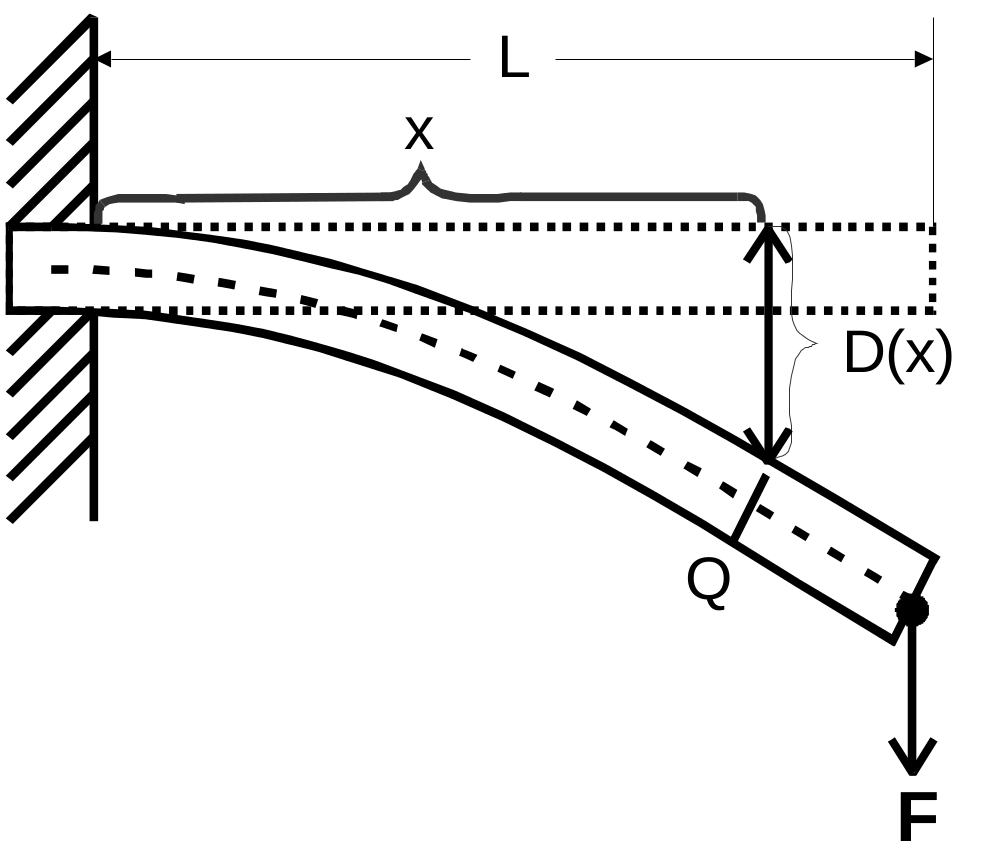
\includegraphics[width=0.5\textwidth]{einseitige.png}
  \caption{Schematische Darstellung der Biegung bei einseitiger Einspannung \cite{sample}.}
  \label{fig:Einseitige_Einspannung}
\end{figure}
Die Durchbiegung $D(x)$ lässt sich ermitteln indem man die Drehmomente aufstellt.
Bei der Biegung wird der eine Teil des Stabs gestaucht und der andere Teil gestreckt.
Der Teil der spannungsfrei ist, wird neutrale Faser genannt und ist in Abbildung
\ref{fig:Einseitige_Einspannung} durch eine gestrichelte Linie angedeutet. Die
wirkenden Kräfte an der Stelle $Q$ sind in Abbildung \ref{fig:Drehmomente} dargestellt.
\begin{figure}[H]
  \centering
  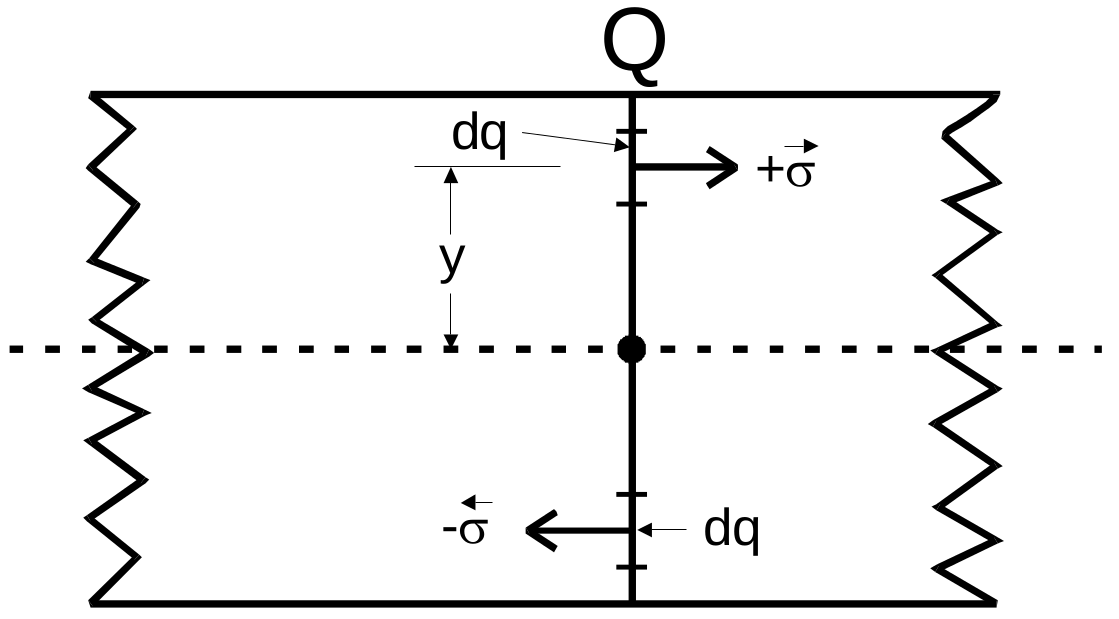
\includegraphics[width=0.5\textwidth]{Drehmomente.png}
  \caption{Darstellung der Drehmomente bei Q \cite{sample}.}
  \label{fig:Drehmomente}
\end{figure}
Die entgegengesetzten Druck- und Zugspannungen sind vom Betrag gleich. Mit Gleichung
\eqref{eqn:moment} lässt sich das Drehmoment $M_\sigma$ berechnen.
\begin{equation}
  M_\sigma=\int_Q y\sigma(y)\text{d}q
  \label{eqn:moment}
\end{equation}
Es stellt sich das Gleichgewicht
\begin{equation*}
  M_F=M_\sigma
\end{equation*}
ein. Das durch die Gewichtskraft des angehängten Gewichts entstehende Drehmoment
$M_F$ ist hierbei gegeben durch
\begin{equation*}
  M_F=F(L-x).
\end{equation*}
Das Gleichtgewicht ist also
\begin{equation}
  \int_Q y\sigma(y)\text{d}q=F(L-x).
\end{equation}
Die Normalspannung ist durch das Hookesche-Gesetz gegeben und ist mit einer Näherung
für geringe Kruvenkrümmungen
\begin{equation*}
  \sigma(y)=E\frac{y}{R}=Ey\frac{\text{d}^2D}{\text{d}x^2}\;,
\end{equation*}
so dass sich das Gleichgewicht als
\begin{equation*}
  E\frac{\text{d}^2D}{\text{d}x^2}\int_Q y^2\text{d}q=F(L_x)
\end{equation*}
schreiben lässt. Das Flächenträgheitsmoment $I$ ist gegeben durch
\begin{equation}
  I=\int_Q y^2 \text{d}q(y)\;.
  \label{eqn:Flaechentraegheitsmoment}
\end{equation}
Wird die Gleichung \eqref{eqn:Flaechentraegheitsmoment} integriert, erhält man die
Gleichung für die Durchbiegung in Abhängigkeit zu Abstand
\begin{equation}
  D(x)=\frac{F}{2EI}\left(Lx^2-\frac{x^3}{3}\right)\;\;\;\;(0\le x \le L)\,.
  \label{eqn:durchbiegung1}
\end{equation}

\subsection{Biegung bei beidseitiger Auflage}
Da beide Enden des Stabes aufliegen, greift nun die Kraft $\frac{F}{2}$ an.
Eine schematische Darstellung ist in Abbildung \ref{fig:Beidseitige_Einspannung}
zu sehen.
\begin{figure}[H]
  \centering
  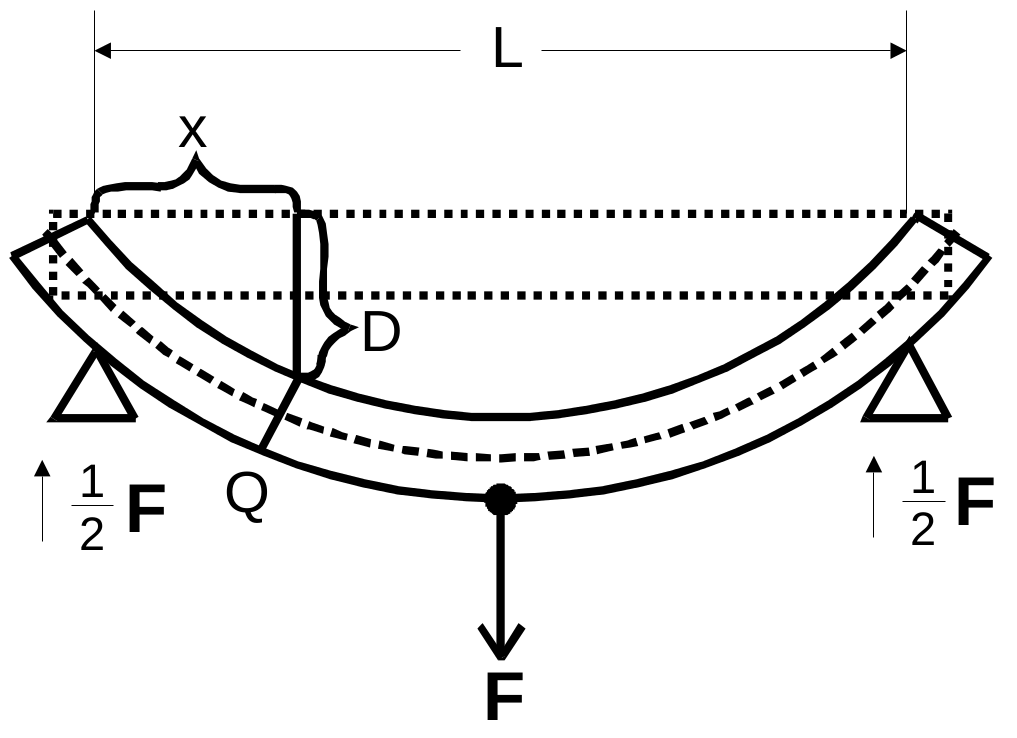
\includegraphics[width=0.5\textwidth]{Beidseitige_Einspannung.png}
  \caption{darstellung der Drehmomente bei Q \cite{sample}.}
  \label{fig:Beidseitige_Einspannung}
\end{figure}
Für die Drehmomente gelten nun
\begin{align}
  \frac{\text{d}^2D}{\text{d}x^2}=&-\frac{F}{EI}\frac{x}{2}\;\;(\text{für}\;0\le x \le \frac{L}{2}\\
  \frac{\text{d}^2D}{\text{d}x^2}=&-\frac{1}{2}\frac{F}{EI}(L-x)\;\; (\text{für}\; \frac{L}{2} \le x \le L)
\end{align}
und damit für die Durchbiegung der linken Hälfte
\begin{equation}
  D(x)=\frac{F}{48EI}\left(3L^2x-4x^3\right)\;\;(\text{für}\;0\le x \le \frac{L}{2})
  \label{eqn:durchbiegung_links}
\end{equation}
und die der rechten Hälfte
\begin{equation}
  D(x)=\frac{F}{48EI}\left(4x^3-12Lx^2+9L^2x-L^3\right)\;\;
  (\text{für}\; \frac{L}{2} \le x \le L).
  \label{eqn:durchbiegung_rechts}
\end{equation}
\cite{sample}
